\documentclass[letterpaper]{article}
\usepackage[utf8]{inputenc}
\usepackage{url}
\usepackage{aaai}
\usepackage{times}
\usepackage{helvet}
\usepackage{courier}
\usepackage{amsmath}
\usepackage{amssymb}
\usepackage{graphicx}

% \frenchspacing
\setlength{\pdfpagewidth}{8.5in}
\setlength{\pdfpageheight}{11in}
\pdfinfo{
/Title (Predicting School Disciplinary Outcomes from Bus Conduct and Referral Data)
/Author (Sindu Chitraju, Samuel Howard, Seif Ilkbarieh, Om Solanki, Andrew Wheeler)}
\setcounter{secnumdepth}{0}  

\begin{document}

% The file aaai.sty is the style file for AAAI Press 
% proceedings, working notes, and technical reports.

% Remove the copyright from the footer
\nocopyright

\title{Predicting School Disciplinary Outcomes from Bus Conduct and Referral Data
}
\author{Sindu Chitraju, Samuel Howard, Seif Ilkbarieh, Om Solanki, Andrew Wheeler\\
Tennessee Technological University
}

\maketitle

\section*{Introduction}

This project focused on identifying patterns in student behavior that 
could help predict major disciplinary actions in schools. We were given 
two datasets from a school district, one with records of student behavior 
on school buses and another with disciplinary referrals during school 
hours. Our main question was whether behavior on the bus, especially 
intentional misconduct, could be used to predict whether a student would 
get a major referral at school.

To explore thiswe performed hypothesis testing and built several models 
including logistic regression, linear regression, and a neural network. 
We wanted to provide the school with both interpretable insights and 
prediction tools that could be helpful for early intervention.

\section*{Data and Preprocessing}

We used two main datasets:

\begin{enumerate}
    \item Bus Conduct Data --- included school name, date, incident type,
    actions taken by the driver, student demographics, and more.

    \item Disciplinary Referral Data --- included date, violation level
    (major/minor), classroom behavior, time of day, and student demographics.
\end{enumerate}

After cleaning both datasets (removing missing values, fixing formatting 
issues, and converting dates and grade levels) we merged them using 
student ID. We also created new features to make the data more useful 
for modelingfor example flags for ``intentional violation'' and binary 
columns for specific behavior keywords.

\section*{Hypothesis Testing}

We ran four hypothesis tests using chi-square tests to check if certain factors were associated with major referrals:

\subsection*{Intentional Bus Violation vs Major Referral}

Result: Statistically significant $(p < 0.001)$. There is a clear 
connection between intentional bus misconduct and receiving a major 
referral.

\subsection*{Gender vs Major Referral}

Result: Not highly significant $(p > 0.001)$.

\subsection*{Grade Level vs Major Referral}

Result: Significant. Higher grade levels were associated with 
proportionally more major referrals.


\subsection*{Time of Day vs Major Referral}

Result: Significant. Certain time periods had more serious behavior 
incidents.

These results supported our idea that student characteristics and past 
behavior (especially on the bus) can be useful indications of more serious 
problems in school. Furthermore, they informed the feature engineering 
and feature selection used in modeling.

\section*{Modeling and Results}

\subsection*{Logistic Regression}

We built a multivariate logistic regression model using student behavior 
features, demographics, and keyword indicators. The model had good 
accuracy and showed that factors like ``fighting,'' ``possession,'' 
and ``intentional violation'' had a strong influence on the likelihood 
of a major referral.

% logistic.png figure
\begin{figure}[htbp]
    \centering
    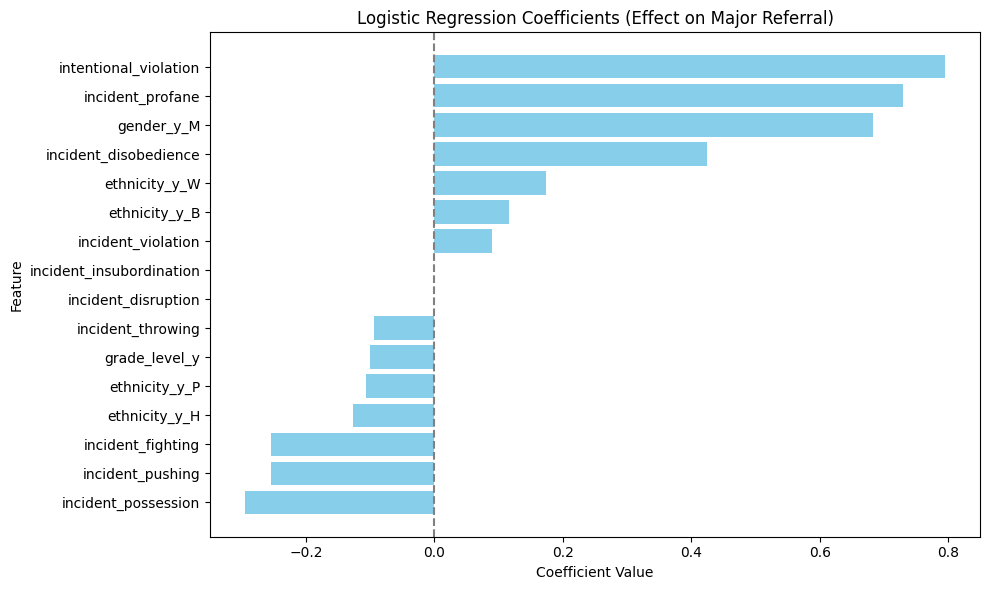
\includegraphics[width=0.4\textwidth]{4220_figures/logistic.png}
    \caption{Logistic regression feature impacts}
    \label{fig:logistic}
\end{figure}

\subsection*{Linear Regression}

We created a severity score (0 = no referral, 1 = minor, 2 = major) 
and used linear regression to predict it. The model wasn't as useful 
for classification, but it gave insights into which behaviors had a 
bigger impact on discipline.

% linear.png figure
\begin{figure}[htbp]
    \centering
    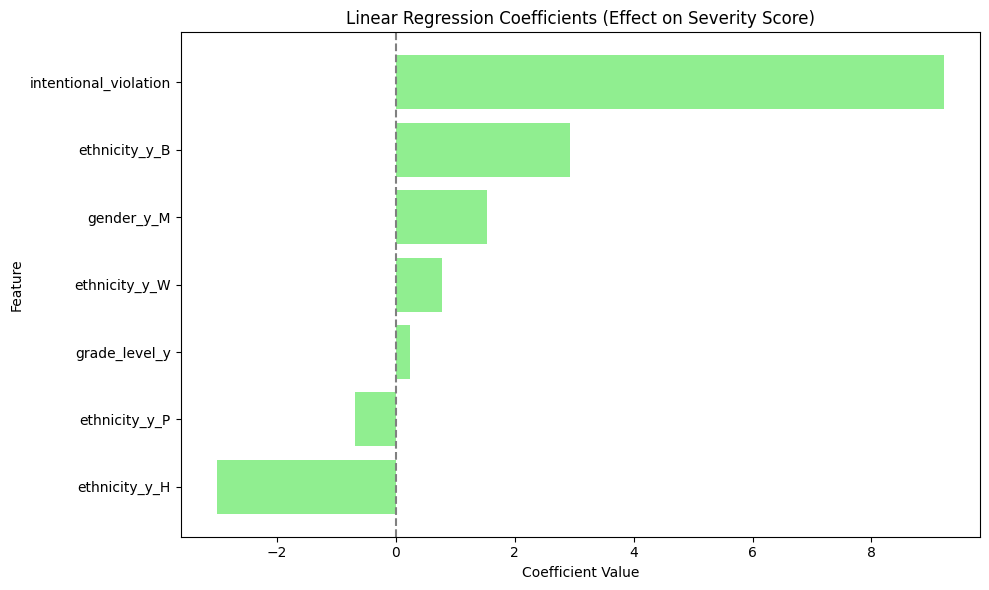
\includegraphics[width=0.4\textwidth]{4220_figures/linear.png}
    \caption{Linear regression feature impacts}
    \label{fig:linear}
\end{figure}

\subsection*{Neural Network}

We built a basic feedforward neural network using TensorFlow. It 
achieved about 83\% accuracy but had a lower recall for predicting 
major referrals (only around 18\%). This means it correctly labeled 
most students but struggled to catch all serious cases.

\subsection*{Random Forest}

We also tried a random forest classifier for comparison. It had 
similar accuracy but slightly better recall (around 25\%), making it 
more balanced than the neural network in identifying major violations.

\subsection*{Comparing The Neural Network to Random Forest}

% nn_vs_rf.png figure
\begin{figure}[htbp]
    \centering
    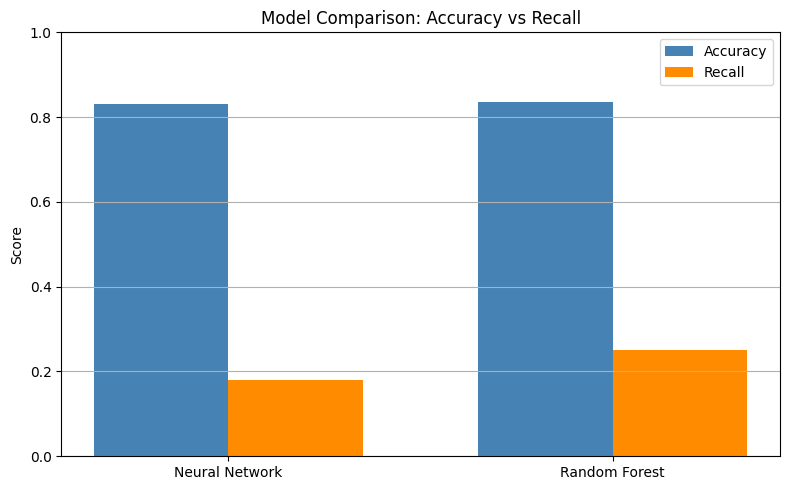
\includegraphics[width=0.4\textwidth]{4220_figures/nn_vs_rf.png}
    \caption{Comparison of the accuracy and recall of the neural network and random forest classifiers}
    \label{fig:linear}
\end{figure}

The neural network, achieved an overall accuracy of approximately 83\%. 
However, its recall for major referrals was substantially lower, at 
around 18\%. This indicates good generalization, but poorer performance
on the positive instances we are looking for.

In contrast, the random forest classifier demonstrated comparable overall 
accuracy, also near 83\%, but achieved a higher recall of approximately 
25\% for major referrals. This performance is more in line with the 
predictions that are valuable in this instance, making it preferred.

Therefore, we conclude that the random forest classifier would be the most 
applicable and useful model of those we tested. Not only does it perform
the best for this application, but it is also more explainable. It can be
inspected to determine why a student might be considered of higher risk
if the prediction it gave yielded negative consequences.

\section*{Interpretation}

The results across all models and tests showed a clear pattern: 
students who had intentional bus violations were much more likely 
to receive major disciplinary actions at school. Logistic regression 
confirmed the strength of this relationship, while linear regression 
and neural nets provided additional support. Some variables, like the 
grade level and ethnicity, also had an influence, which may be worth 
exploring further in future research or school policy discussions.

\section*{Conclusion}

This project helped answer the school's main question: yes, bus 
behavior especially intentional misbehavior can help predict serious 
school discipline outcomes. Our analysis showed that it's possible to 
build models that provide early warning signs using existing data. For 
future work, we recommend trying time-series models that track 
students behavior over the semester or year to make predictions 
even more accurate.

\end{document}